% ---------------------------------------------------
\chapter{Basic-Block-Level Code Replication (BBLCR)}
\label{chap:bblcr}
% ---------------------------------------------------

\section*{Overview}
Basic-Block-Level Code Replication (BBLCR) refines the principles of FLCR by moving
validation and redirection from function boundaries down to individual control-flow blocks.
Each basic block—defined as a straight-line sequence of instructions ending in a branch or jump—
is treated as an independently verifiable unit.  If a fault corrupts one block, execution can
skip over the damaged block and continue using a valid counterpart instead of discarding the
entire function.

While FLCR isolates faults between functions, BBLCR extends that protection inside functions,
enabling the program to survive corruption at a much finer granularity.

% ---------------------------------------------------
\section*{Mechanism}
BBLCR introduces runtime validation and redirection for intra-function control flow.
Every branch or jump instruction is rewritten so that its destination is resolved through
a runtime lookup structure known as the \textbf{Block Table (BTab)}, which records the
currently validated address of each replicated basic block.
This structure performs the same role as the ITab in FLCR but operates one level deeper.

\subsection*{Static Metadata}
Static metadata describes all replicated basic blocks and is finalized after linking,
when instruction addresses and block boundaries are fully known.

\begin{itemize}
  \item \textbf{Block Address Table:} lists the base address of every block replica within each function.
  \item \textbf{Block Size Table:} records the byte length of each block, used for hash computation.
  \item \textbf{Block Hash Table:} contains reference checksums for every replica, generated after linking and relocation.
\end{itemize}

\subsection*{Runtime Dynamic Data}
At runtime, two structures maintain the validated execution state:

\begin{itemize}
  \item \textbf{Block Table (BTab):} maps each block identifier (BID) to its validated target.
        All conditional and unconditional branches resolve through this table.
  \item \textbf{Branch Map (BMap):} used for indirect or computed jumps; associates the original
        target address with the verified replica.  It supports control transfers that are not statically known.
\end{itemize}

\subsection*{Core Components}
BBLCR reuses the same validation framework as FLCR but applies it at the basic-block level.

\begin{itemize}
  \item \textbf{Validator:} computes and checks the hash of every basic-block replica.
  \item \textbf{Selector:} chooses a valid replica for each block; if none are valid, it defaults to the first replica.
  \item \textbf{Metadata Initializer:} runs once at startup, invoking the Selector and Validator to populate BTab and BMap.
  \item \textbf{Edge Resolver:} executes only at runtime branch sites that were originally indirect or computed jumps,
        searching BMap for the validated target.
\end{itemize}

\subsection*{Branch Transformation}
Every branch and jump instruction is rewritten to route through the runtime indirection
layer, ensuring that all control flow enters only validated basic blocks.
Each transformation consults the \textbf{Block Table (BTab)} for statically known edges,
or the \textbf{Branch Map (BMap)} for computed or indirect edges.

\begin{table}[h!]
  \centering
  \renewcommand{\arraystretch}{1.2}
  \begin{tabularx}{\linewidth}{|l|X|X|}
    \hline
    \textbf{Branch Type} & \textbf{Original} & \textbf{Transformed} \\ \hline
    Unconditional branch &
    \texttt{jmp L1} &
    \texttt{load target ← BTab[BID\_L1]} \newline
    \texttt{jmp target} \\ \hline

    Unconditional branch (indirect) &
    \texttt{jmp *ptr} &
    \texttt{target ← resolver(ptr)} \newline
    \texttt{jmp target} \\ \hline

    Conditional branch &
    \texttt{br cond, L\_T, L\_F} &
    \texttt{load T ← BTab[BID\_T]} \newline
    \texttt{load F ← BTab[BID\_F]} \newline
    \texttt{sel target ← cond ? T : F} \newline
    \texttt{br target} \\ \hline

    Conditional branch (indirect) &
    \texttt{br cond, *ptr\_T, *ptr\_F} &
    \texttt{T ← resolver(ptr\_T)} \newline
    \texttt{F ← resolver(ptr\_F)} \newline
    \texttt{sel target ← cond ? T : F} \newline
    \texttt{br target} \\ \hline
  \end{tabularx}
  \caption{Unified BBLCR branch transformation for unconditional, conditional,
           and indirect control transfers.}
  \label{tab:bblcr-transform}
\end{table}

This unified transformation guarantees that all control-flow edges—direct, conditional,
and indirect—are redirected through validated structures.
Because basic blocks are smaller than functions, faults can be contained more precisely,
allowing recovery within individual routines.

These transformations rely on the presence of \textbf{indirect branch instructions}
within the instruction set architecture.
Such instructions (e.g., ARM \texttt{BX}, RISC-V \texttt{JALR}, x86 \texttt{jmp *reg})
allow branch destinations to be computed dynamically at runtime, enabling seamless
redirection to validated replicas while preserving the original control-flow structure.

Architectures that lack indirect branching (for example, those that only permit fixed
or PC-relative targets) must emulate this behavior using additional control logic.
In such systems, the compiler introduces explicit control or dispatcher blocks,
as described in the next section.

% ---------------------------------------------------
\subsection*{Control and Target Blocks (Systems Without Indirect Branch Support)}
The control and target block distinction arises only on architectures that \emph{lack}
native indirect branch instructions.  In these systems, branches and jumps cannot take
a computed destination directly, so BBLCR must emulate redirection through additional
control logic.

Under such conditions, each original basic block divides into two roles:

\begin{itemize}
  \item \textbf{Target blocks:} contain the executable program logic and act as the true
        branch destinations under validation.
  \item \textbf{Control blocks:} inserted to perform runtime redirection and validation
        lookups through the \textbf{BTab} or \textbf{BMap} structures.
\end{itemize}

Whenever a target block is replicated, a control block must precede it to handle redirection.
If that control block later becomes the target of another branch, an additional control
block must be introduced in front of it—creating recursive expansion and increasing
control-block density.  This expansion raises instruction count and weakens spatial locality
between related code regions.

Ideally, a target block and its associated control block would remain \textbf{contiguous in memory},
forming a small, self-contained protection region.  In practice, compiler scheduling, padding,
and link-time reordering scatter these blocks throughout the binary, making contiguity rare.
Target and control blocks often become \textbf{discontinuous}, preventing validation as a single region.

Because of this discontinuity, it becomes impossible to maintain \textbf{block groups}—sets of
related blocks that could be invalidated together if one fails validation.  Inserted control
stubs fragment the layout, separating targets that once shared a logical flow.  Group invalidation
therefore becomes unsafe, since invalidating a ``group'' might also remove unrelated control code.

Consequently, protection boundaries must terminate at the \textbf{target block}.
The control block functions as a trusted redirector but cannot itself be validated in the same way,
as its position and linkage may vary across compilations.  Only the target block can be considered
clean and fault-free under the validation model.

This structural limitation highlights a key tradeoff of fine-grained replication:
as granularity increases, isolation improves, but on systems without indirect branch support,
compiler layout and control fragmentation make contiguous protection increasingly difficult.

% ---------------------------------------------------
\section*{Control-Flow Structure and Replication}
The structure of BBLCR can be illustrated using the simple loop example shown in
Figure~\ref{fig:bblcr-combined}.
Subfigure~(a) depicts the baseline control-flow graph of a typical \texttt{for} loop,
composed of five basic blocks: \textbf{Entry}, \textbf{Condition}, \textbf{Body},
\textbf{Increment}, and \textbf{Exit}. Control flows cyclically between the
\textbf{Condition} and \textbf{Body} blocks until the loop terminates.

Subfigure~(b) shows the same loop after transformation under BBLCR.
Each basic block is independently replicated, and all control-flow edges are redirected
through the validated \textbf{Block Table (BTab)}.
Conditional branches dynamically resolve both their true and false targets through BTab,
ensuring that every transition occurs only between verified replicas.

\begin{figure}[t]
  \centering
  \begin{subfigure}[t]{0.47\linewidth}
    \centering
    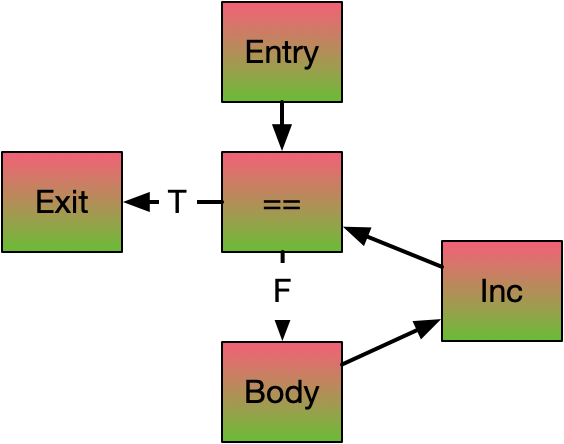
\includegraphics[width=\linewidth]{Chapter-8/figs/bblcr-baseline.png}
    \caption{Baseline control-flow graph for a simple \texttt{for} loop showing
             \textbf{Entry}, \textbf{Condition}, \textbf{Body}, \textbf{Increment},
             and \textbf{Exit} blocks.}
    \label{fig:bblcr-baseline}
  \end{subfigure}
  \hfill
  \begin{subfigure}[t]{0.47\linewidth}
    \centering
    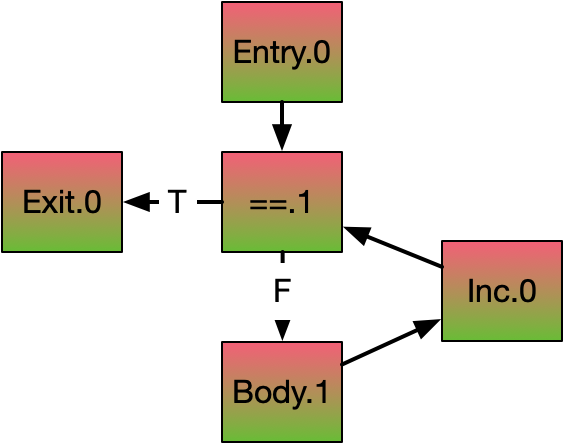
\includegraphics[width=\linewidth]{Chapter-8/figs/bblcr-replicated.png}
    \caption{Replicated control-flow graph under BBLCR. Each branch and jump resolves
             through the validated \textbf{BTab}, allowing the system to skip corrupted
             basic blocks and continue through verified replicas.}
    \label{fig:bblcr-replicated}
  \end{subfigure}
  \caption{Comparison of baseline and BBLCR-transformed control flow for a simple loop:
           (a) baseline function layout, (b) replicated layout with runtime redirection.}
  \label{fig:bblcr-combined}
\end{figure}

This combined view highlights two central aspects of BBLCR:
\begin{enumerate}
  \item \textbf{Granularity:} validation occurs at each basic-block boundary,
        allowing localized fault containment within a function.
  \item \textbf{Edge indirection:} every branch and jump is resolved through runtime
        tables, preventing entry into unvalidated code.
\end{enumerate}

In larger applications, each basic block operates as a relocatable unit of verified logic,
connected through fault-tolerant control edges that maintain functional continuity
even in the presence of localized corruption.

% ---------------------------------------------------
\section*{Execution Flow}
At runtime, initialization proceeds identically to FLCR.
The \textbf{Metadata Initializer} invokes the \textbf{Selector} and \textbf{Validator}
to populate the \textbf{BTab} and \textbf{BMap} before execution begins.
After initialization, every intra-function branch and jump passes through the validated indirection layer.

In a baseline program, branches connect directly between blocks with no runtime validation.
Under BBLCR, each branch or jump first consults \textbf{BTab} (for static edges)
or \textbf{BMap} (for computed targets) before transferring control.
This design allows the program to skip corrupted paths dynamically while continuing
through validated replicas.

% ---------------------------------------------------
\section*{Limit Study}
The Basic-Block-Level Code Replication (BBLCR) limit study evaluates the practical
benefits of fine-grained replication in a controlled, minimal environment.
Unlike previous large-scale benchmark studies, this experiment isolates a single
loop construct to observe the effects of corruption and recovery in detail.

\subsection*{Setup}
Figure~\ref{fig:bblcr-limit-flow} illustrates the experimental flow.
A shared library containing a simple \texttt{for}-loop function was used as the test
subject.  The library was independently instrumented for three configurations:
\textbf{Baseline}, \textbf{FLCR}, and \textbf{BBLCR}.

Bit-flip faults were randomly injected into the library’s executable image to
simulate instruction corruption.  The corrupted shared object was then dynamically
loaded and executed by a host program.  During execution, the selection and validation
routines (when enabled) verified and redirected control to validated replicas.
Program output was compared against a known reference output to determine whether
execution remained correct.

\begin{figure}[t]
  \centering
  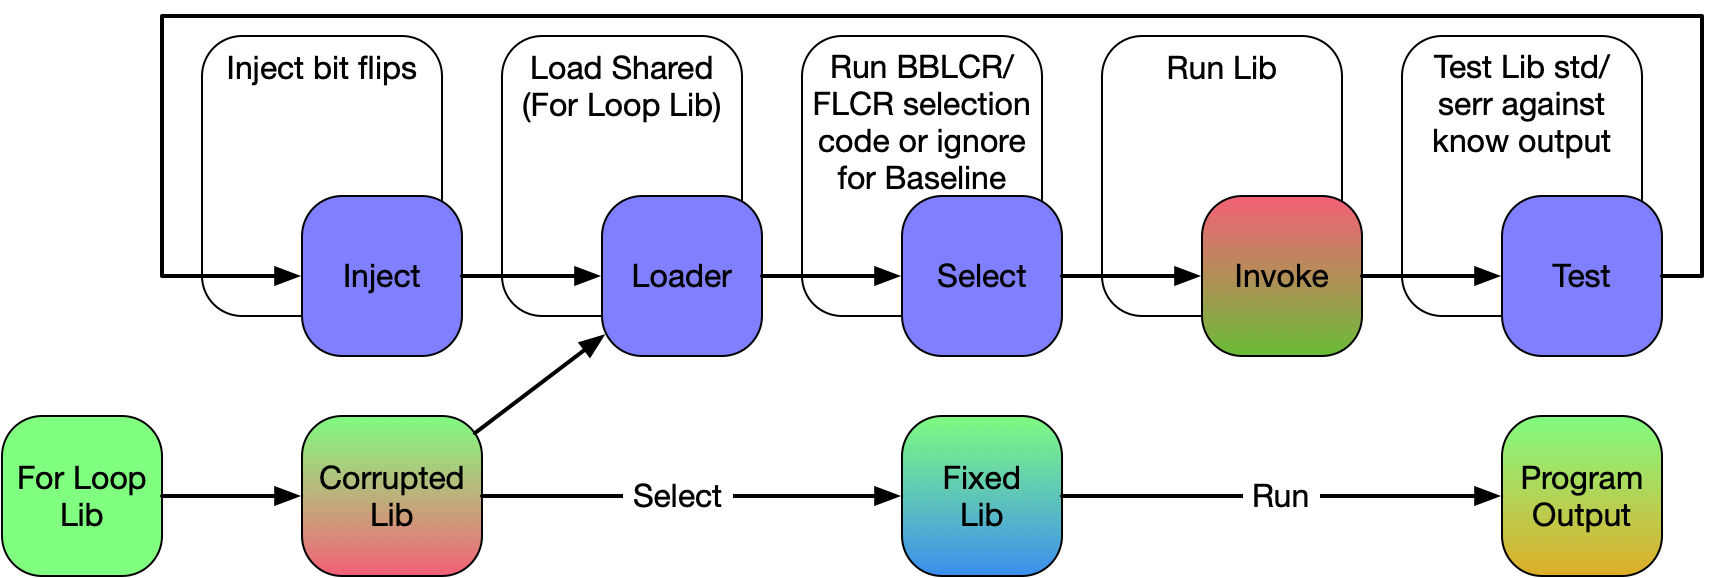
\includegraphics[width=\linewidth]{Chapter-8/figs/bblcr-limit-flow.png}
  \caption{Limit study experimental flow for Baseline, FLCR, and BBLCR configurations.
           A shared library implementing a simple \texttt{for}-loop is corrupted,
           dynamically loaded, and executed.  The resulting output is validated
           against a known reference to measure reliability.}
  \label{fig:bblcr-limit-flow}
\end{figure}

\subsection*{Results}
The fault injection campaign was repeated across multiple corruption levels,
each representing an increasing density of random bit flips within the shared object.
For the \textbf{Baseline}, any corruption within the loop body typically resulted
in immediate program failure or incorrect output.

With \textbf{FLCR}, function-level replication successfully recovered from
corruptions that affected a subset of functions, but failures persisted when
multiple corrupted basic blocks appeared within the same function body.
\textbf{BBLCR} eliminated this limitation by validating and redirecting at the
basic-block level, maintaining correct operation even when isolated loop blocks
were corrupted.

\subsection*{Interpretation}
This experiment demonstrates that fine-grained replication significantly improves
software survivability under instruction faults, even in minimal programs.
BBLCR’s local validation and redirection allow execution to bypass individual
corrupted blocks, providing functional continuity where FLCR and Baseline fail.

However, this improvement comes with increased metadata overhead and runtime
complexity, even in a simple workload.  The benefit therefore depends on the
application domain: systems with compact, time-critical code may favor coarser
granularity, while those demanding resilience at any cost—such as recovery loops
or embedded control kernels—stand to gain the most from BBLCR.

% ---------------------------------------------------
\section*{Summary}
This chapter introduced Basic-Block-Level Code Replication (BBLCR),
a fine-grained replication mechanism that operates at the level of individual
basic blocks. BBLCR extends the concept of runtime indirection from functions
to intra-function control flow, using a per-block lookup structure to
validate and redirect execution at each branch boundary.

The design allows the system to isolate faults within specific control-flow
segments, improving fault survivability compared to both FLCR and Baseline.
Through the loop-based limit study, BBLCR maintained correct operation even
when corruption occurred inside individual loop blocks, demonstrating effective
containment at the basic-block level.

However, finer granularity also introduced practical constraints.
Additional control blocks and validation lookups increased metadata overhead,
and compiler scheduling often scattered related blocks, preventing contiguous
protection regions. Only the target block could be considered truly validated,
while the surrounding control logic remained structurally exposed.

In summary, BBLCR achieves the highest fault isolation among the replication
models but exposes tradeoffs in layout continuity and runtime complexity.
Its results form the final stage of the granularity spectrum explored in this work.
The next chapter revisits all limit study results together, comparing
reliability trends and overhead across RLCR, FLCR, and BBLCR configurations.